

\subsection{Diskussion}
\label{sub:diskussion_3}
Die vorliegen Ergebnisse zeigen, dass keine meiner Forschungshypothesen auf die Gruppe von Untersuchungspersonen zutrifft. 

Einen Grund sehe ich wie in Abschnitt~\ref{sub:diskussion_1} und Abschnitt~\ref{sub:diskussion_2} in der Operationalisierung des Flow-Erlebens durch die \ac{FKS} beim Laufen. Die beschriebene Studie zeigt, dass eine Überforderung von mehreren Untersuchungspersonen als optimal bewertet wurde. Dieses führt zu hohen Werten bei der Absorbiertheit bei hoher mittlerer \ac{HR}, was gleichzeitig zu niedrigen Werten bei der kardio-lokomotorischen Phasensynchronisation führt. Dieser Sachverhalt ist durch die Betrachtung der von mir nachträglich durchgeführten subjektiven Einteilung nach physischer Beanspruchung deutlich (vgl. Abbildung~\ref{fig:5_20_mittelwert_vergleich} A, B, C). Bei überfordert zeigt der Mittelwertvergleich die höchsten Mittelwerte bei der mittleren \ac{HR} und dem Bewegungsaufwand, dennoch ist der Wert der $\bigtriangleup$Absorbiertheit im Mittel am höchsten. Lassen wir die Bewertung der Absorbiertheit bei überfordert außen vor, verdeutlicht Abbildung~\ref{fig:5_20_mittelwert_vergleich}, dass ein optimaler Zustand beim Laufen am positivsten von den Untersuchungspersonen bewertet wurde, die eine optimale mittlere \ac{HR} und die höchsten Werte der kardio-lokomotorischen Phasensynchronisation besaßen.

\begin{figure}
	% Created by tikzDevice version 0.10.1 on 2016-06-17 11:20:51
% !TEX encoding = UTF-8 Unicode
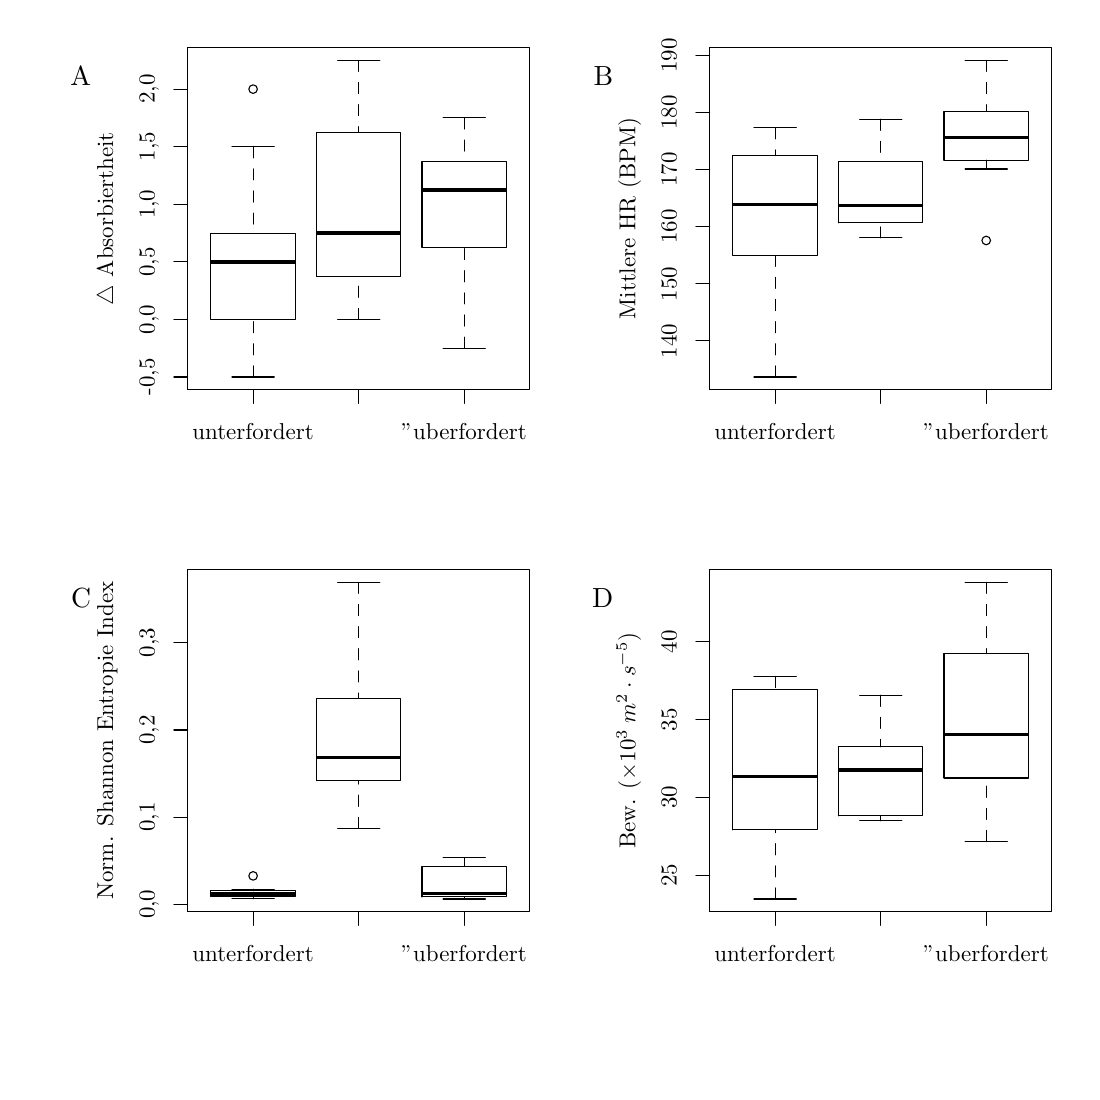
\begin{tikzpicture}[x=1pt,y=1pt]
\definecolor{fillColor}{RGB}{255,255,255}
\path[use as bounding box,fill=fillColor,fill opacity=0.00] (0,0) rectangle (377.25,377.25);
\begin{scope}
\path[clip] ( 57.82,246.44) rectangle (181.40,370.02);
\definecolor{drawColor}{RGB}{0,0,0}

\path[draw=drawColor,line width= 1.2pt,line join=round] ( 66.21,292.63) -- ( 96.72,292.63);

\path[draw=drawColor,line width= 0.4pt,dash pattern=on 4pt off 4pt ,line join=round,line cap=round] ( 81.46,251.02) -- ( 81.46,271.82);

\path[draw=drawColor,line width= 0.4pt,dash pattern=on 4pt off 4pt ,line join=round,line cap=round] ( 81.46,334.24) -- ( 81.46,303.03);

\path[draw=drawColor,line width= 0.4pt,line join=round,line cap=round] ( 73.84,251.02) -- ( 89.09,251.02);

\path[draw=drawColor,line width= 0.4pt,line join=round,line cap=round] ( 73.84,334.24) -- ( 89.09,334.24);

\path[draw=drawColor,line width= 0.4pt,line join=round,line cap=round] ( 66.21,271.82) --
	( 96.72,271.82) --
	( 96.72,303.03) --
	( 66.21,303.03) --
	( 66.21,271.82);

\path[draw=drawColor,line width= 0.4pt,line join=round,line cap=round] ( 81.46,355.04) circle (  1.55);

\path[draw=drawColor,line width= 1.2pt,line join=round] (104.35,303.03) -- (134.86,303.03);

\path[draw=drawColor,line width= 0.4pt,dash pattern=on 4pt off 4pt ,line join=round,line cap=round] (119.61,271.82) -- (119.61,287.43);

\path[draw=drawColor,line width= 0.4pt,dash pattern=on 4pt off 4pt ,line join=round,line cap=round] (119.61,365.45) -- (119.61,339.44);

\path[draw=drawColor,line width= 0.4pt,line join=round,line cap=round] (111.98,271.82) -- (127.24,271.82);

\path[draw=drawColor,line width= 0.4pt,line join=round,line cap=round] (111.98,365.45) -- (127.24,365.45);

\path[draw=drawColor,line width= 0.4pt,line join=round,line cap=round] (104.35,287.43) --
	(134.86,287.43) --
	(134.86,339.44) --
	(104.35,339.44) --
	(104.35,287.43);

\path[draw=drawColor,line width= 1.2pt,line join=round] (142.49,318.63) -- (173.01,318.63);

\path[draw=drawColor,line width= 0.4pt,dash pattern=on 4pt off 4pt ,line join=round,line cap=round] (157.75,261.42) -- (157.75,297.83);

\path[draw=drawColor,line width= 0.4pt,dash pattern=on 4pt off 4pt ,line join=round,line cap=round] (157.75,344.64) -- (157.75,329.04);

\path[draw=drawColor,line width= 0.4pt,line join=round,line cap=round] (150.12,261.42) -- (165.38,261.42);

\path[draw=drawColor,line width= 0.4pt,line join=round,line cap=round] (150.12,344.64) -- (165.38,344.64);

\path[draw=drawColor,line width= 0.4pt,line join=round,line cap=round] (142.49,297.83) --
	(173.01,297.83) --
	(173.01,329.04) --
	(142.49,329.04) --
	(142.49,297.83);
\end{scope}
\begin{scope}
\path[clip] (  0.00,  0.00) rectangle (377.25,377.25);
\definecolor{drawColor}{RGB}{0,0,0}

\path[draw=drawColor,line width= 0.4pt,line join=round,line cap=round] ( 81.46,246.44) -- (157.75,246.44);

\path[draw=drawColor,line width= 0.4pt,line join=round,line cap=round] ( 81.46,246.44) -- ( 81.46,241.46);

\path[draw=drawColor,line width= 0.4pt,line join=round,line cap=round] (119.61,246.44) -- (119.61,241.46);

\path[draw=drawColor,line width= 0.4pt,line join=round,line cap=round] (157.75,246.44) -- (157.75,241.46);

\node[text=drawColor,anchor=base,inner sep=0pt, outer sep=0pt, scale=  0.83] at ( 81.46,228.51) {unterfordert};

\node[text=drawColor,anchor=base,inner sep=0pt, outer sep=0pt, scale=  0.83] at (157.75,228.51) {"uberfordert};

\path[draw=drawColor,line width= 0.4pt,line join=round,line cap=round] ( 57.82,251.02) -- ( 57.82,355.04);

\path[draw=drawColor,line width= 0.4pt,line join=round,line cap=round] ( 57.82,251.02) -- ( 52.84,251.02);

\path[draw=drawColor,line width= 0.4pt,line join=round,line cap=round] ( 57.82,271.82) -- ( 52.84,271.82);

\path[draw=drawColor,line width= 0.4pt,line join=round,line cap=round] ( 57.82,292.63) -- ( 52.84,292.63);

\path[draw=drawColor,line width= 0.4pt,line join=round,line cap=round] ( 57.82,313.43) -- ( 52.84,313.43);

\path[draw=drawColor,line width= 0.4pt,line join=round,line cap=round] ( 57.82,334.24) -- ( 52.84,334.24);

\path[draw=drawColor,line width= 0.4pt,line join=round,line cap=round] ( 57.82,355.04) -- ( 52.84,355.04);

\node[text=drawColor,rotate= 90.00,anchor=base,inner sep=0pt, outer sep=0pt, scale=  0.83] at ( 45.86,251.02) {-0,5};

\node[text=drawColor,rotate= 90.00,anchor=base,inner sep=0pt, outer sep=0pt, scale=  0.83] at ( 45.86,271.82) {0,0};

\node[text=drawColor,rotate= 90.00,anchor=base,inner sep=0pt, outer sep=0pt, scale=  0.83] at ( 45.86,292.63) {0,5};

\node[text=drawColor,rotate= 90.00,anchor=base,inner sep=0pt, outer sep=0pt, scale=  0.83] at ( 45.86,313.43) {1,0};

\node[text=drawColor,rotate= 90.00,anchor=base,inner sep=0pt, outer sep=0pt, scale=  0.83] at ( 45.86,334.24) {1,5};

\node[text=drawColor,rotate= 90.00,anchor=base,inner sep=0pt, outer sep=0pt, scale=  0.83] at ( 45.86,355.04) {2,0};
\end{scope}
\begin{scope}
\path[clip] (  0.00,188.62) rectangle (188.62,377.25);
\definecolor{drawColor}{RGB}{0,0,0}

\node[text=drawColor,rotate= 90.00,anchor=base,inner sep=0pt, outer sep=0pt, scale=  0.83] at ( 30.92,308.23) {$\bigtriangleup$ Absorbiertheit};
\end{scope}
\begin{scope}
\path[clip] (  0.00,  0.00) rectangle (377.25,377.25);
\definecolor{drawColor}{RGB}{0,0,0}

\path[draw=drawColor,line width= 0.4pt,line join=round,line cap=round] ( 57.82,246.44) --
	(181.40,246.44) --
	(181.40,370.02) --
	( 57.82,370.02) --
	( 57.82,246.44);

\node[text=drawColor,anchor=base east,inner sep=0pt, outer sep=0pt, scale=  1.00] at ( 22.96,356.44) {A};
\end{scope}
\begin{scope}
\path[clip] (246.44,246.44) rectangle (370.02,370.02);
\definecolor{drawColor}{RGB}{0,0,0}

\path[draw=drawColor,line width= 1.2pt,line join=round] (254.83,313.25) -- (285.35,313.25);

\path[draw=drawColor,line width= 0.4pt,dash pattern=on 4pt off 4pt ,line join=round,line cap=round] (270.09,251.02) -- (270.09,294.96);

\path[draw=drawColor,line width= 0.4pt,dash pattern=on 4pt off 4pt ,line join=round,line cap=round] (270.09,341.04) -- (270.09,331.00);

\path[draw=drawColor,line width= 0.4pt,line join=round,line cap=round] (262.46,251.02) -- (277.72,251.02);

\path[draw=drawColor,line width= 0.4pt,line join=round,line cap=round] (262.46,341.04) -- (277.72,341.04);

\path[draw=drawColor,line width= 0.4pt,line join=round,line cap=round] (254.83,294.96) --
	(285.35,294.96) --
	(285.35,331.00) --
	(254.83,331.00) --
	(254.83,294.96);

\path[draw=drawColor,line width= 1.2pt,line join=round] (292.97,313.10) -- (323.49,313.10);

\path[draw=drawColor,line width= 0.4pt,dash pattern=on 4pt off 4pt ,line join=round,line cap=round] (308.23,301.29) -- (308.23,306.72);

\path[draw=drawColor,line width= 0.4pt,dash pattern=on 4pt off 4pt ,line join=round,line cap=round] (308.23,344.17) -- (308.23,328.92);

\path[draw=drawColor,line width= 0.4pt,line join=round,line cap=round] (300.60,301.29) -- (315.86,301.29);

\path[draw=drawColor,line width= 0.4pt,line join=round,line cap=round] (300.60,344.17) -- (315.86,344.17);

\path[draw=drawColor,line width= 0.4pt,line join=round,line cap=round] (292.97,306.72) --
	(323.49,306.72) --
	(323.49,328.92) --
	(292.97,328.92) --
	(292.97,306.72);

\path[draw=drawColor,line width= 1.2pt,line join=round] (331.12,337.59) -- (361.63,337.59);

\path[draw=drawColor,line width= 0.4pt,dash pattern=on 4pt off 4pt ,line join=round,line cap=round] (346.37,326.16) -- (346.37,329.34);

\path[draw=drawColor,line width= 0.4pt,dash pattern=on 4pt off 4pt ,line join=round,line cap=round] (346.37,365.45) -- (346.37,346.95);

\path[draw=drawColor,line width= 0.4pt,line join=round,line cap=round] (338.75,326.16) -- (354.00,326.16);

\path[draw=drawColor,line width= 0.4pt,line join=round,line cap=round] (338.75,365.45) -- (354.00,365.45);

\path[draw=drawColor,line width= 0.4pt,line join=round,line cap=round] (331.12,329.34) --
	(361.63,329.34) --
	(361.63,346.95) --
	(331.12,346.95) --
	(331.12,329.34);

\path[draw=drawColor,line width= 0.4pt,line join=round,line cap=round] (346.37,300.35) circle (  1.55);
\end{scope}
\begin{scope}
\path[clip] (  0.00,  0.00) rectangle (377.25,377.25);
\definecolor{drawColor}{RGB}{0,0,0}

\path[draw=drawColor,line width= 0.4pt,line join=round,line cap=round] (270.09,246.44) -- (346.37,246.44);

\path[draw=drawColor,line width= 0.4pt,line join=round,line cap=round] (270.09,246.44) -- (270.09,241.46);

\path[draw=drawColor,line width= 0.4pt,line join=round,line cap=round] (308.23,246.44) -- (308.23,241.46);

\path[draw=drawColor,line width= 0.4pt,line join=round,line cap=round] (346.37,246.44) -- (346.37,241.46);

\node[text=drawColor,anchor=base,inner sep=0pt, outer sep=0pt, scale=  0.83] at (270.09,228.51) {unterfordert};

\node[text=drawColor,anchor=base,inner sep=0pt, outer sep=0pt, scale=  0.83] at (346.37,228.51) {"uberfordert};

\path[draw=drawColor,line width= 0.4pt,line join=round,line cap=round] (246.44,264.07) -- (246.44,367.18);

\path[draw=drawColor,line width= 0.4pt,line join=round,line cap=round] (246.44,264.07) -- (241.46,264.07);

\path[draw=drawColor,line width= 0.4pt,line join=round,line cap=round] (246.44,284.69) -- (241.46,284.69);

\path[draw=drawColor,line width= 0.4pt,line join=round,line cap=round] (246.44,305.32) -- (241.46,305.32);

\path[draw=drawColor,line width= 0.4pt,line join=round,line cap=round] (246.44,325.94) -- (241.46,325.94);

\path[draw=drawColor,line width= 0.4pt,line join=round,line cap=round] (246.44,346.56) -- (241.46,346.56);

\path[draw=drawColor,line width= 0.4pt,line join=round,line cap=round] (246.44,367.18) -- (241.46,367.18);

\node[text=drawColor,rotate= 90.00,anchor=base,inner sep=0pt, outer sep=0pt, scale=  0.83] at (234.49,264.07) {140};

\node[text=drawColor,rotate= 90.00,anchor=base,inner sep=0pt, outer sep=0pt, scale=  0.83] at (234.49,284.69) {150};

\node[text=drawColor,rotate= 90.00,anchor=base,inner sep=0pt, outer sep=0pt, scale=  0.83] at (234.49,305.32) {160};

\node[text=drawColor,rotate= 90.00,anchor=base,inner sep=0pt, outer sep=0pt, scale=  0.83] at (234.49,325.94) {170};

\node[text=drawColor,rotate= 90.00,anchor=base,inner sep=0pt, outer sep=0pt, scale=  0.83] at (234.49,346.56) {180};

\node[text=drawColor,rotate= 90.00,anchor=base,inner sep=0pt, outer sep=0pt, scale=  0.83] at (234.49,367.18) {190};
\end{scope}
\begin{scope}
\path[clip] (188.62,188.62) rectangle (377.25,377.25);
\definecolor{drawColor}{RGB}{0,0,0}

\node[text=drawColor,rotate= 90.00,anchor=base,inner sep=0pt, outer sep=0pt, scale=  0.83] at (219.55,308.23) {Mittlere HR (BPM)};
\end{scope}
\begin{scope}
\path[clip] (  0.00,  0.00) rectangle (377.25,377.25);
\definecolor{drawColor}{RGB}{0,0,0}

\path[draw=drawColor,line width= 0.4pt,line join=round,line cap=round] (246.44,246.44) --
	(370.02,246.44) --
	(370.02,370.02) --
	(246.44,370.02) --
	(246.44,246.44);

\node[text=drawColor,anchor=base east,inner sep=0pt, outer sep=0pt, scale=  1.00] at (211.58,356.44) {B};
\end{scope}
\begin{scope}
\path[clip] ( 57.82, 57.82) rectangle (181.40,181.40);
\definecolor{drawColor}{RGB}{0,0,0}

\path[draw=drawColor,line width= 1.2pt,line join=round] ( 66.21, 64.22) -- ( 96.72, 64.22);

\path[draw=drawColor,line width= 0.4pt,dash pattern=on 4pt off 4pt ,line join=round,line cap=round] ( 81.46, 62.50) -- ( 81.46, 63.38);

\path[draw=drawColor,line width= 0.4pt,dash pattern=on 4pt off 4pt ,line join=round,line cap=round] ( 81.46, 65.91) -- ( 81.46, 65.36);

\path[draw=drawColor,line width= 0.4pt,line join=round,line cap=round] ( 73.84, 62.50) -- ( 89.09, 62.50);

\path[draw=drawColor,line width= 0.4pt,line join=round,line cap=round] ( 73.84, 65.91) -- ( 89.09, 65.91);

\path[draw=drawColor,line width= 0.4pt,line join=round,line cap=round] ( 66.21, 63.38) --
	( 96.72, 63.38) --
	( 96.72, 65.36) --
	( 66.21, 65.36) --
	( 66.21, 63.38);

\path[draw=drawColor,line width= 0.4pt,line join=round,line cap=round] ( 81.46, 70.75) circle (  1.55);

\path[draw=drawColor,line width= 1.2pt,line join=round] (104.35,113.43) -- (134.86,113.43);

\path[draw=drawColor,line width= 0.4pt,dash pattern=on 4pt off 4pt ,line join=round,line cap=round] (119.61, 87.91) -- (119.61,105.14);

\path[draw=drawColor,line width= 0.4pt,dash pattern=on 4pt off 4pt ,line join=round,line cap=round] (119.61,176.82) -- (119.61,134.89);

\path[draw=drawColor,line width= 0.4pt,line join=round,line cap=round] (111.98, 87.91) -- (127.24, 87.91);

\path[draw=drawColor,line width= 0.4pt,line join=round,line cap=round] (111.98,176.82) -- (127.24,176.82);

\path[draw=drawColor,line width= 0.4pt,line join=round,line cap=round] (104.35,105.14) --
	(134.86,105.14) --
	(134.86,134.89) --
	(104.35,134.89) --
	(104.35,105.14);

\path[draw=drawColor,line width= 1.2pt,line join=round] (142.49, 64.30) -- (173.01, 64.30);

\path[draw=drawColor,line width= 0.4pt,dash pattern=on 4pt off 4pt ,line join=round,line cap=round] (157.75, 62.39) -- (157.75, 63.15);

\path[draw=drawColor,line width= 0.4pt,dash pattern=on 4pt off 4pt ,line join=round,line cap=round] (157.75, 77.30) -- (157.75, 74.20);

\path[draw=drawColor,line width= 0.4pt,line join=round,line cap=round] (150.12, 62.39) -- (165.38, 62.39);

\path[draw=drawColor,line width= 0.4pt,line join=round,line cap=round] (150.12, 77.30) -- (165.38, 77.30);

\path[draw=drawColor,line width= 0.4pt,line join=round,line cap=round] (142.49, 63.15) --
	(173.01, 63.15) --
	(173.01, 74.20) --
	(142.49, 74.20) --
	(142.49, 63.15);
\end{scope}
\begin{scope}
\path[clip] (  0.00,  0.00) rectangle (377.25,377.25);
\definecolor{drawColor}{RGB}{0,0,0}

\path[draw=drawColor,line width= 0.4pt,line join=round,line cap=round] ( 81.46, 57.82) -- (157.75, 57.82);

\path[draw=drawColor,line width= 0.4pt,line join=round,line cap=round] ( 81.46, 57.82) -- ( 81.46, 52.84);

\path[draw=drawColor,line width= 0.4pt,line join=round,line cap=round] (119.61, 57.82) -- (119.61, 52.84);

\path[draw=drawColor,line width= 0.4pt,line join=round,line cap=round] (157.75, 57.82) -- (157.75, 52.84);

\node[text=drawColor,anchor=base,inner sep=0pt, outer sep=0pt, scale=  0.83] at ( 81.46, 39.89) {unterfordert};

\node[text=drawColor,anchor=base,inner sep=0pt, outer sep=0pt, scale=  0.83] at (157.75, 39.89) {"uberfordert};

\path[draw=drawColor,line width= 0.4pt,line join=round,line cap=round] ( 57.82, 60.49) -- ( 57.82,154.98);

\path[draw=drawColor,line width= 0.4pt,line join=round,line cap=round] ( 57.82, 60.49) -- ( 52.84, 60.49);

\path[draw=drawColor,line width= 0.4pt,line join=round,line cap=round] ( 57.82, 91.99) -- ( 52.84, 91.99);

\path[draw=drawColor,line width= 0.4pt,line join=round,line cap=round] ( 57.82,123.48) -- ( 52.84,123.48);

\path[draw=drawColor,line width= 0.4pt,line join=round,line cap=round] ( 57.82,154.98) -- ( 52.84,154.98);

\node[text=drawColor,rotate= 90.00,anchor=base,inner sep=0pt, outer sep=0pt, scale=  0.83] at ( 45.86, 60.49) {0,0};

\node[text=drawColor,rotate= 90.00,anchor=base,inner sep=0pt, outer sep=0pt, scale=  0.83] at ( 45.86, 91.99) {0,1};

\node[text=drawColor,rotate= 90.00,anchor=base,inner sep=0pt, outer sep=0pt, scale=  0.83] at ( 45.86,123.48) {0,2};

\node[text=drawColor,rotate= 90.00,anchor=base,inner sep=0pt, outer sep=0pt, scale=  0.83] at ( 45.86,154.98) {0,3};
\end{scope}
\begin{scope}
\path[clip] (  0.00,  0.00) rectangle (188.62,188.62);
\definecolor{drawColor}{RGB}{0,0,0}

\node[text=drawColor,rotate= 90.00,anchor=base,inner sep=0pt, outer sep=0pt, scale=  0.83] at ( 30.92,119.61) {Norm. Shannon Entropie Index};
\end{scope}
\begin{scope}
\path[clip] (  0.00,  0.00) rectangle (377.25,377.25);
\definecolor{drawColor}{RGB}{0,0,0}

\path[draw=drawColor,line width= 0.4pt,line join=round,line cap=round] ( 57.82, 57.82) --
	(181.40, 57.82) --
	(181.40,181.40) --
	( 57.82,181.40) --
	( 57.82, 57.82);

\node[text=drawColor,anchor=base east,inner sep=0pt, outer sep=0pt, scale=  1.00] at ( 22.96,167.82) {C};
\end{scope}
\begin{scope}
\path[clip] (246.44, 57.82) rectangle (370.02,181.40);
\definecolor{drawColor}{RGB}{0,0,0}

\path[draw=drawColor,line width= 1.2pt,line join=round] (254.83,106.72) -- (285.35,106.72);

\path[draw=drawColor,line width= 0.4pt,dash pattern=on 4pt off 4pt ,line join=round,line cap=round] (270.09, 62.39) -- (270.09, 87.39);

\path[draw=drawColor,line width= 0.4pt,dash pattern=on 4pt off 4pt ,line join=round,line cap=round] (270.09,142.78) -- (270.09,138.16);

\path[draw=drawColor,line width= 0.4pt,line join=round,line cap=round] (262.46, 62.39) -- (277.72, 62.39);

\path[draw=drawColor,line width= 0.4pt,line join=round,line cap=round] (262.46,142.78) -- (277.72,142.78);

\path[draw=drawColor,line width= 0.4pt,line join=round,line cap=round] (254.83, 87.39) --
	(285.35, 87.39) --
	(285.35,138.16) --
	(254.83,138.16) --
	(254.83, 87.39);

\path[draw=drawColor,line width= 1.2pt,line join=round] (292.97,108.97) -- (323.49,108.97);

\path[draw=drawColor,line width= 0.4pt,dash pattern=on 4pt off 4pt ,line join=round,line cap=round] (308.23, 90.66) -- (308.23, 92.44);

\path[draw=drawColor,line width= 0.4pt,dash pattern=on 4pt off 4pt ,line join=round,line cap=round] (308.23,136.05) -- (308.23,117.37);

\path[draw=drawColor,line width= 0.4pt,line join=round,line cap=round] (300.60, 90.66) -- (315.86, 90.66);

\path[draw=drawColor,line width= 0.4pt,line join=round,line cap=round] (300.60,136.05) -- (315.86,136.05);

\path[draw=drawColor,line width= 0.4pt,line join=round,line cap=round] (292.97, 92.44) --
	(323.49, 92.44) --
	(323.49,117.37) --
	(292.97,117.37) --
	(292.97, 92.44);

\path[draw=drawColor,line width= 1.2pt,line join=round] (331.12,121.94) -- (361.63,121.94);

\path[draw=drawColor,line width= 0.4pt,dash pattern=on 4pt off 4pt ,line join=round,line cap=round] (346.37, 83.14) -- (346.37,106.13);

\path[draw=drawColor,line width= 0.4pt,dash pattern=on 4pt off 4pt ,line join=round,line cap=round] (346.37,176.82) -- (346.37,151.09);

\path[draw=drawColor,line width= 0.4pt,line join=round,line cap=round] (338.75, 83.14) -- (354.00, 83.14);

\path[draw=drawColor,line width= 0.4pt,line join=round,line cap=round] (338.75,176.82) -- (354.00,176.82);

\path[draw=drawColor,line width= 0.4pt,line join=round,line cap=round] (331.12,106.13) --
	(361.63,106.13) --
	(361.63,151.09) --
	(331.12,151.09) --
	(331.12,106.13);
\end{scope}
\begin{scope}
\path[clip] (  0.00,  0.00) rectangle (377.25,377.25);
\definecolor{drawColor}{RGB}{0,0,0}

\path[draw=drawColor,line width= 0.4pt,line join=round,line cap=round] (270.09, 57.82) -- (346.37, 57.82);

\path[draw=drawColor,line width= 0.4pt,line join=round,line cap=round] (270.09, 57.82) -- (270.09, 52.84);

\path[draw=drawColor,line width= 0.4pt,line join=round,line cap=round] (308.23, 57.82) -- (308.23, 52.84);

\path[draw=drawColor,line width= 0.4pt,line join=round,line cap=round] (346.37, 57.82) -- (346.37, 52.84);

\node[text=drawColor,anchor=base,inner sep=0pt, outer sep=0pt, scale=  0.83] at (270.09, 39.89) {unterfordert};

\node[text=drawColor,anchor=base,inner sep=0pt, outer sep=0pt, scale=  0.83] at (346.37, 39.89) {"uberfordert};

\path[draw=drawColor,line width= 0.4pt,line join=round,line cap=round] (246.44, 71.00) -- (246.44,155.29);

\path[draw=drawColor,line width= 0.4pt,line join=round,line cap=round] (246.44, 71.00) -- (241.46, 71.00);

\path[draw=drawColor,line width= 0.4pt,line join=round,line cap=round] (246.44, 99.10) -- (241.46, 99.10);

\path[draw=drawColor,line width= 0.4pt,line join=round,line cap=round] (246.44,127.20) -- (241.46,127.20);

\path[draw=drawColor,line width= 0.4pt,line join=round,line cap=round] (246.44,155.29) -- (241.46,155.29);

\node[text=drawColor,rotate= 90.00,anchor=base,inner sep=0pt, outer sep=0pt, scale=  0.83] at (234.49, 71.00) {25};

\node[text=drawColor,rotate= 90.00,anchor=base,inner sep=0pt, outer sep=0pt, scale=  0.83] at (234.49, 99.10) {30};

\node[text=drawColor,rotate= 90.00,anchor=base,inner sep=0pt, outer sep=0pt, scale=  0.83] at (234.49,127.20) {35};

\node[text=drawColor,rotate= 90.00,anchor=base,inner sep=0pt, outer sep=0pt, scale=  0.83] at (234.49,155.29) {40};
\end{scope}
\begin{scope}
\path[clip] (188.62,  0.00) rectangle (377.25,188.62);
\definecolor{drawColor}{RGB}{0,0,0}

\node[text=drawColor,rotate= 90.00,anchor=base,inner sep=0pt, outer sep=0pt, scale=  0.83] at (219.55,119.61) {Bew. ($\times 10^3 \: m^2 \cdot s^{-5}$)};
\end{scope}
\begin{scope}
\path[clip] (  0.00,  0.00) rectangle (377.25,377.25);
\definecolor{drawColor}{RGB}{0,0,0}

\path[draw=drawColor,line width= 0.4pt,line join=round,line cap=round] (246.44, 57.82) --
	(370.02, 57.82) --
	(370.02,181.40) --
	(246.44,181.40) --
	(246.44, 57.82);

\node[text=drawColor,anchor=base east,inner sep=0pt, outer sep=0pt, scale=  1.00] at (211.58,167.82) {D};
\end{scope}
\end{tikzpicture}

	\caption[Mittelwertvergleich (Studie: Laufen)]{Mittelwertvergleich der finalen Studie zum Flow-Erleben beim Laufen -- unterfordert, optimal, überfordert. (A) $\bigtriangleup$Absorbiertheit; (B) Mittlere HR; (C) Mittlerer normalisierter Shannon Entropie Index; (D) Bewegungsaufwand. Quelle: Eigene Darstellung \\ \hspace{\textwidth}\emph{Anmerkung}: Bew. = Bewegungsaufwand\\ \hspace{\textwidth}$\bigtriangleup$ Wert berechnet durch die Subtraktion des Baseline-Wertes.}
	\label{fig:5_20_mittelwert_vergleich}
\end{figure}

Ich hinterfrage die Zusammenstellung der Untersuchungspersonen grundsätzlich, da die Gruppe überwiegend aus Fußballern bestand. Mehrere Teilnehmer konnten keine kardio-lokomotorischen Phasensynchronisation herstellen, die die Untersuchungsperson aus der ersten Fallstudie weniger oder mehr in sechs von sechs Sitzungen herstellen konnte. Das begründe ich durch die sporadische Lauferfahrung von Fußballern. Darum fand ich keinen interindividuellen quadratischen Zusammenhang in Form einer umgedrehten U-Kurve wie in Abschnitt~\ref{sub:diskussion_1} und Abschnitt~\ref{sub:diskussion_2} zwischen kardio-lokomotorischen Phasensynchronisation und mittlerer \ac{HR}.

Allgemein zeigt die Operationalisierung durch die \ac{FKS} große Mängel beim Faktor Absorbiertheit in meiner Studie, da das Item "`Ich fühle mich optimal beansprucht."' positiver bewertet wurde als die anderen drei Items des Faktors. Das probeweise Weglassen des Items ergab aber keine Verbesserung der Ergebnisse. \citet{Henk2014} erhielt in seiner Studie vergleichbare Ergebnisse bei der Operationalisierung des Flow-Erlebens durch strukturierte Interviews und der \ac{FKS}. Nichtsdestotrotz halte ich die \ac{FKS} nicht für ein geeignetes Instrument für die Operationalisierung des Flow-Erlebens beim Laufen, da Untersuchungspersonen die Aussagen missverstehen oder individuell interpretieren können. Es bleibt unklar, wie die Antwort in Form eines Kreuzes an einer Stelle der Skala zustande kommt. Die Operationalisierung des Flow-Erlebens durch ein zwar zeitaufwendigeres strukturiertes Interview besitzt bei der korrekten Anwendung einen höheren und präziseren Informationsgehalt über das Flow-Erleben. 

Ich sehe die kardio-lokomotorische Phasensynchronisation und den Bewegungsaufwand aufgrund der Nachbetrachtung als Erfolg versprechende Kandidaten für ein implizites Messverfahren des Flow-Erlebens an. Die kardio-lokomotorische Phasensynchronisation betrachte ich als Voraussetzung für Flow-Erleben und einen personenindividuellen messbaren Unterschied des Bewegungsaufwands ohne eine Laufgeschwindigkeitsänderung als Folge des Flow-Erlebens beim Laufen an. 

\section{Zusammenfassung}
\label{sec:zusammenfassung_5}

Von drei Studien dienten die ersten beiden Fallstudien mit jeweils einer Untersuchungsperson zur Hypothesenbildung und testeten Annahmen für den Einzelfall. In der dritten Studie mit 36 Untersuchungsteilnehmern testete ich die aufgestellten Forschungshypothesen. Die Ergebnisse der drei Studien bestätigen statistisch keine der von mir im Vorfeld getroffenen Annahmen. Dennoch geben sie mir Hinweise auf:

\begin{itemize}
	\item einen personenindividuellen quadratischen Zusammenhang in Form einer umgedrehten U-Kurve zwischen Flow-Erleben und mittlere HR
	\item einen personenindividuellen positiven linearen Zusammenhang zwischen Flow-Erleben und kardio-lokomotorischer Phasensynchronisation
	\item einen personenindividuellen negativen linearen Zusammenhang von Flow-Erleben und Bewegungsaufwand
	\item einen allgemeingültigen positiven linearen Zusammenhang zwischen Flow-Erleben und kardio-lokomotorischer Phasensynchronisation
\end{itemize}

Alle Zusammenhänge benötigen zusätzliche Untersuchungen mit hinreichenden befriedigenden Ergebnissen, bevor einer der Kandidaten als implizites Messverfahren des Flow-Erlebens automatisiert und in Echtzeit mobil von jemandem einzusetzen ist. 